\section{Expliquer les différents types de signaux et donner des exemples}

Il existe plusieurs types de signaux étudiés en posturographie, à l'aide de différents instruments.

\subsection{Les forces et moments}

Les forces sont les interactions mécaniques exercées par les pieds du patient sur la \textbf{surface d'une plateforme de mesure}.
Ces forces sont mesurées dans les trois directions de l'espace : 
\begin{itemize}
  \item $F_x$ : force horizontale le long de l'axe $x$
  \item $F_y$ : force horizontale le long de l'axe $y$ 
  \item $F_z$ : force verticale, perpendiculaire à la surface (poids corporel ou force de gravité)
\end{itemize}
Ici, les forces $F_x$ et $F_y$ caractérisent les efforts de contrôle postural pour maintenir l'équilibre 
en gérant les déplacement latéraux ($x$) et avant-arrière ($y$).
$F_z$ caractérise la force exercée par le poids du corps sur la plateforme. Elle varie 
lors des mouvements dynamiques (e.g. sauts, marches ou transitions).

Les moments sont les forces de rotations générées autour des axes principaux de la plateforme.
Ils mesurent les rotations produites par les forces appliquées par le corps.
Les moments sont aussi mesurés dans les trois directions de l'espace : 

\begin{itemize}
  \item $M_x$ : moment autour de l'axe $x$, reflétant les rotations dans le plan frontal (inclinaison latérale du corps)
  \item $M_y$ : moment autour de l'axe $y$, indiquant les rotations dans le plan sagittal (basculement avant-arrière du corps)
  \item $M_z$ : moment autour de l'axe $z$, mesurant les rotations 
\end{itemize}

Les moments donnent des informations sur les ajustements posturaux, comme un déséquilibre latéral ($M_x$) 
ou une bascule avant-arrière ($M_y$) peut indiquer des stratégies de compensation. La torsion du corps ($M_z$) en réponse à un mouvement ou à une perturbation.

Les résultantes égales et opposées des forces agissant sur la masse corporelle s'appliquent respectivement au centre de gravité et au centre de pression.

L'équilibre est atteint à la condition que ces deux points soient alignés sur la même verticale.

\begin{figure}[h]
  \centering
  \begin{subfigure}[b]{0.45\textwidth}
    \centering
    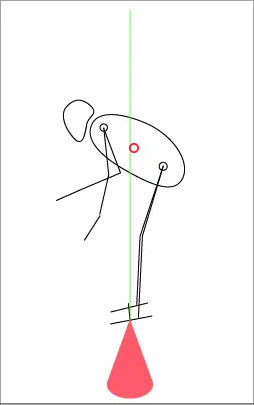
\includegraphics[height=5cm]{images/tactique-cdg.png}
    \caption{Tactique CDG}
    \label{fig:tactique_cdg}
  \end{subfigure}
  \hfill
  \begin{subfigure}[b]{0.45\textwidth}
    \centering
    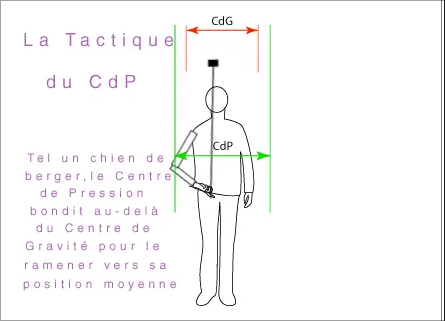
\includegraphics[height=5cm]{images/tactique-cdp.png}
    \caption{Tactique CDP}
    \label{fig:tactique_cdp}
  \end{subfigure}
  \caption{Différentes tactiques}
  \label{fig:2_tactiques}
\end{figure}

Ces mesures servent à l'analyse des oscillations posturales (statiques et dynamiques) et permettent d'évaluer la répartition du poids entre les deux pieds.

\subsection{Accélération et vitesses angulaires (Centrales inertielles, IMU)}

Les \textbf{accélérations} mesurent les variations de vitesse des segments corporels dans les trois axes de l'espace ($x$,$y$,$z$). 
Ces mesures sont réalisées par des \textbf{accéléromètres}, qui détectent les forces d'accélération appliquées au corps ou à ses \textit{segments}. 
Cela permet d'identifier les changements rapides dans dynamique corporelle, comme lors d'un déséquilibre ou d'une activité physique intense.

Les \textbf{vitesses angulaires} mesurent les rotations des segments corporels autour des axes principaux (pitch, roll, yaw). 
Capturées par des gyroscopes, ces données renseignent sur l’amplitude et la vitesse des mouvements rotatifs (par exemple, une rotation du tronc ou de la tête).
On s'en sert pour analyser les stratégies d'ajustement postural ou les mouvements complexes.

Avec ces deux types de signaux, on peut en déduire la \textit{stabilité dynamique}, qui permet de comprendre les micro-enregistrements permettant le maintien de l'équilibre dans des environnements dynamiques, et la mesure de la qualité des réponses posturales à des perturbations externes.
Ces signaux permettent également de suivre précisément les déplacements et rotations des segments corporels (les membres, le tronc, la tête...) afin d'évaluer les asymétries ou déséquilibres.

Ces mesures sont utilisées dans diverses situations.
Elles sont utilisées pour mesurer les progrès dans la récupération posturale ou locomotrice (e.g. après une blessure, un AVC).
Elles permettent également d'analyser les performances athlétiques des mouvements dans des environnements non contrôlés,
comme les terrains de sport ou les espaces naturel athlétiques des mouvements dans des environnements non contrôlés, comme les terrains de sport ou les espaces naturels.

Des machines spécialisées existent pour suivre et mesurer ces signaux:
\begin{itemize}
  \item \textbf{Xsens MTw Awinda} : capture les accélérations et vitesses angulaires pour \\ une analyse cinématique complète.
  \item \textbf{Noraxon MyoMotion} : fournit des mesures détaillées des mouvements segmentaires en \\ intégrant des capteurs inertiels.
  \item \textbf{IMU portables (Shimmer, Delsys)} : capteurs légers fixés sur le tronc, les membres ou la tête pour des analyses mobiles.
\end{itemize}

\begin{figure}[ht]
  \begin{center}
    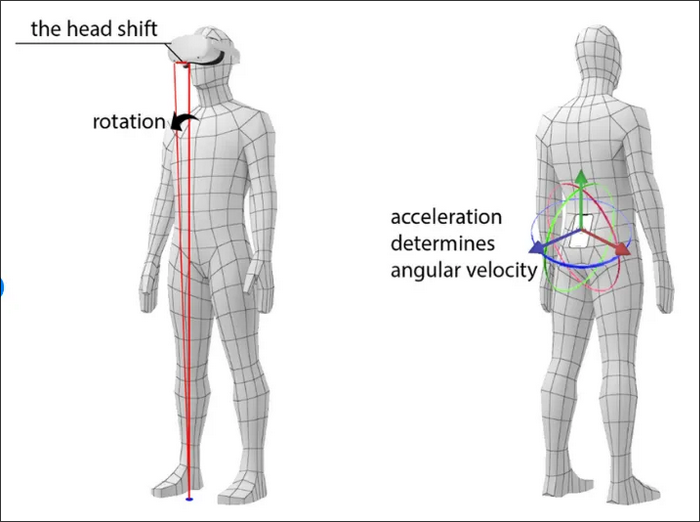
\includegraphics[width=0.5\textwidth]{images/legende.png}
  \end{center}
  \caption{Légende à trouver}\label{fig:legende}
\end{figure}

\subsection{Pressions plantaires (Systèmes de baropodométrie)}

Les \textbf{pressions plantaires} mesurent la répartition des forces sous les pieds au niveau des zones d'appui. 
Ces pressions sont capturées par des capteurs disposés sur une surface ou intégrés dans des semelles.
Ces mesures permettent d'identifier les points de pression maximale et minimale, fournissant des données sur la statique et la dynamique du pied.

Les \textbf{centres de pression} sont calculés à partir des variations de pression. Ils reflètent les ajustements dynamiques de la posture en réponse aux déséquilibres.

Les mesures de ces signaux nous permettent de \textbf{cartographier} les zones d'appui de visualiser les charges appliquées sur les pieds. 
On peut alors identifier les zones à risque de pathologie (comme l'hallux valgus ou la fasciite plantaire).
On peut également analyser la dynamique du pied, c'est-à-dire analyser les phases d'appui et de propulsion pendant la marche ou la course.
L'évaluation des déséquilibres ou anomalies dans la distribution des forces est alors possible.

Ces études sont appliquées en podologie et orthopédie, pour détecter les troubles plantaires ou les anomalies posturales.
Elles sont aussi utilisées pour suivre les progrès post-blessures ou post-chirurgie de patients.
Enfin, on peut aussi les mener dans le but d'optimiser les performances athlétiques en analysant les impacts au sol.

Ces mesures sont rendues possibles grâce à des machines spécialisées : 
\begin{itemize}
  \item \textbf{Tekscan F-scan} : plateforme baropodométrique pour analyse en statique et dynamique
  \item \textbf{Zebris FDM} : Système baropodométrique avancé utilisé en rééducation et recherche.
  \item \textbf{Semelles capturant les pressions (Moticon)} : Capteurs intégrés pour une analyse mobile.
\end{itemize}

\begin{figure}[H]
  \centering
  \begin{subfigure}[b]{0.4\linewidth}
    \centering
    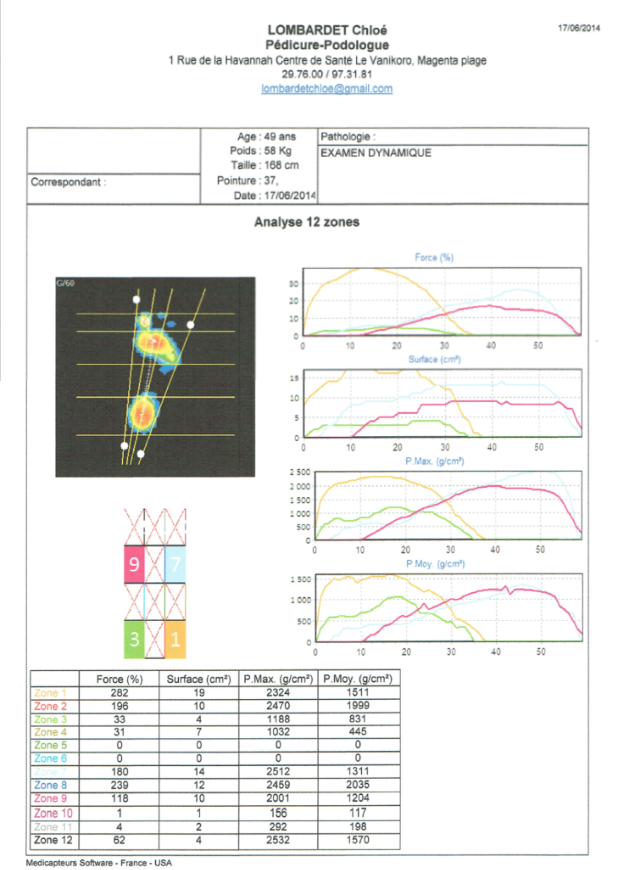
\includegraphics[width=\textwidth, height=10cm]{images/analyse_12_zone.png}
    \caption{Analyse en 12 zones}
    \label{fig:analyse_12_zone}
  \end{subfigure}
  \hspace{0.03\textwidth}
  \begin{subfigure}[b]{0.4\linewidth}
    \centering
    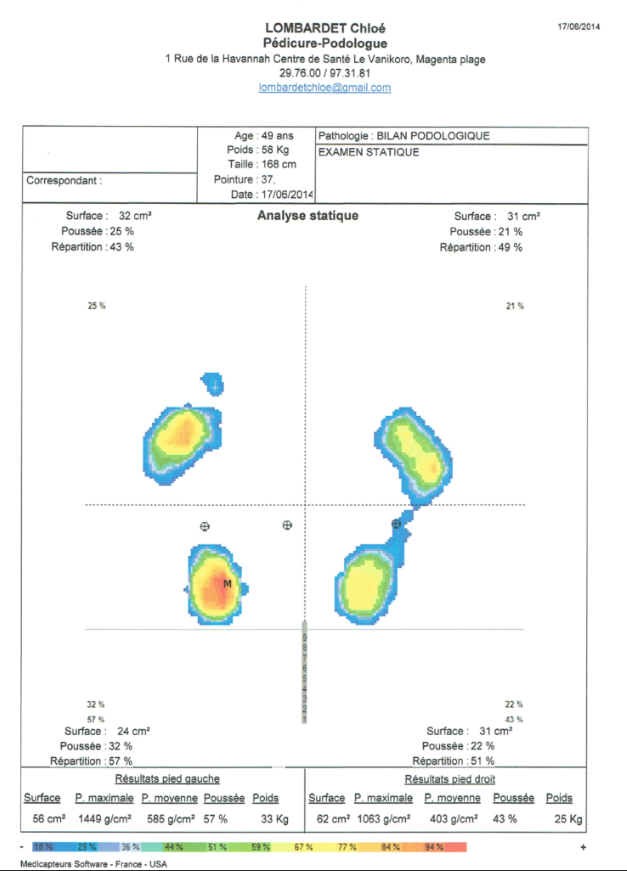
\includegraphics[width=\textwidth, height=10cm]{images/analyse_statique.png}
    \caption{Analyse statique}
    \label{fig:analyse_statique}
  \end{subfigure}
  \begin{subfigure}[b]{0.4\linewidth}
    \centering
    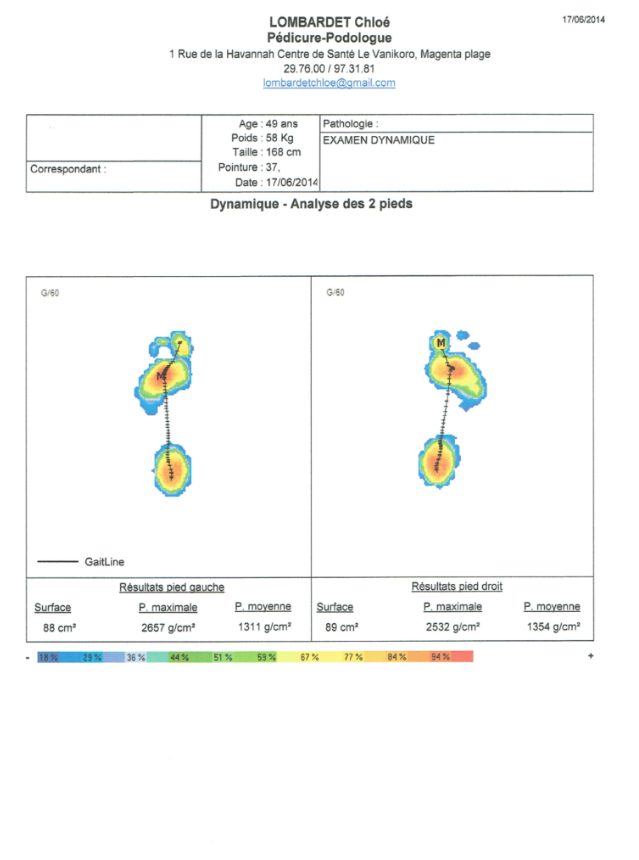
\includegraphics[width=\textwidth, height=10cm]{images/analyse_2_pieds.png}
    \caption{Analyse des deux pieds}
    \label{fig:analyse_2_pieds}
  \end{subfigure}
  \caption{Rapports de différents types d'analyse}
  \label{fig:3_type_analyse}
\end{figure}

\subsection{Potentiels électriques musculaires (EMG - Électromyographie)}

Les \textbf{potentiels électriques musculaires} sont utilisés pour mesurer l'activité électrique
générée par les muscles lors de leurs contractions. Ces signaux sont enregistrés avec des électrodes de surface ou intramusculaires.
Les signaux EMG reflètent l'intensité et la durée d'activation musculaire.
Ces signaux sont influencés par le recrutement des fibres musculaires et leur fréquence de décharge.
Les données EMG permettent de suivre l'ordre d'activation des muscles et leur coordination.

L'étude de ces données nous permet de mesurer l'effort des groupes musculaires en réponse à des tâches posturales ou locomotrices.
Elle nous permet également de mieux identifier les synergies musculaires et les déséquilibres entre muscles agonistes et antagonistes.

Ces analyses sont notamment réalisées dans le cadre de détection des troubles neuromusculaires (par exemple, faiblesse musculaire ou spasticité).
Elles sont aussi performées dans le but d'analyser des stratégies musculaires afin d'optimiser les performances.
Finalement, ces données sont aussi récoltées pour le suivi de la récupération musculaire après des blessures ou des interventions chirurgicales.
 
Ces mesures sont rendues possibles grâce à des machines spécialisées : 
\begin{itemize}
  \item \textbf{Delsys Trigno} : fournit des enregistrements sans fil haute résolution de l’activité musculaire.
  \item \textbf{Noraxon Ultium EMG} : Utilisé pour une analyse avancée en sport et en biomécanique.
  \item \textbf{BTS FREEEMG} : Un système sans fil permettant une analyse complète de l’activation musculaire.
\end{itemize}

\begin{figure}[ht]
  \centering
  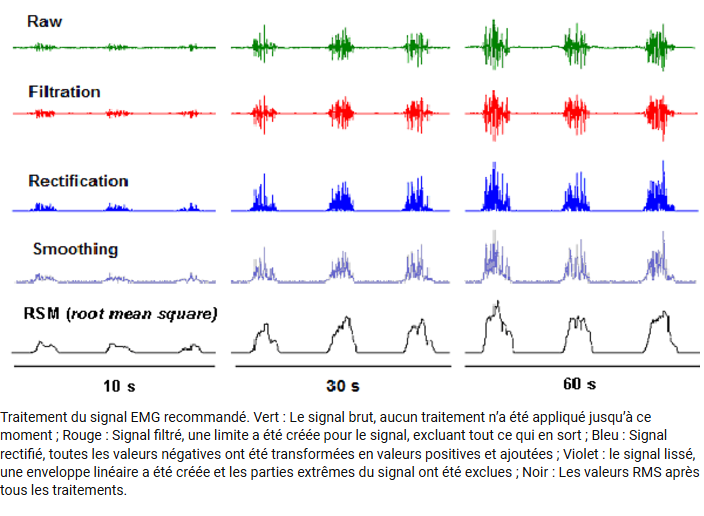
\includegraphics[width=0.5\textwidth]{images/emg.png}
  \caption{Exemple de signal EMG relevé}\label{fig:emg}
\end{figure}


\subsection{Trajectoires segmentaires (systèmes de capture vidéo 3D)}

Les \textbf{trajectoires tridimensionnelles} sont des signaux utilisés pour mesurer les déplacement des segments corporels (membres, tronc, tête) dans les trois axes de l'espace.
Il sont capturés à l'aide de caméras et de marqueurs placés sur le corps.

Les \textbf{angles articulaires} sont calculés à partir de trajectoires segmentaires pour évaluer les amplitudes de mouvement.

À l'aide de ces deux signaux, on peut recréer une cinématique détaillée, qui est un suivi précis des mouvements segmentaires et des angles articulaires.
Ils permettent aussi d'évaluer les asymétries ou anomalies de mouvements, utiles dans le diagnostic des troubles musculo-squelettiques.

L'analyse de ces signaux est effectuée en recherche clinique, dans l'étude de la cinématique du mouvement d'un patient atteint de troubles neurologiques ou orthopédique.
Elle est également faite à des fins d'optimisation des mouvements d'un athlète, afin d'améliorer sa performance.
Elle est aussi utilisée pour suivre les progrès post-blessure ou post-chirurgie d'un patient en réhabilitation.

Ces analyses sont rendues possible grâce à ces machines spécialisées : 
\begin{itemize}
  \item \textbf{Vicon} : système de capture de mouvements de haute précision pour une analyse en 3D.
  \item \textbf{OptiTrack} : fournit des solutions flexibles pour la cinématique du mouvement.
  \item \textbf{Qualisys} : système avancé pour capturer et analyser les mouvements complexes.
\end{itemize}

\begin{figure}[ht]
  \begin{center}
    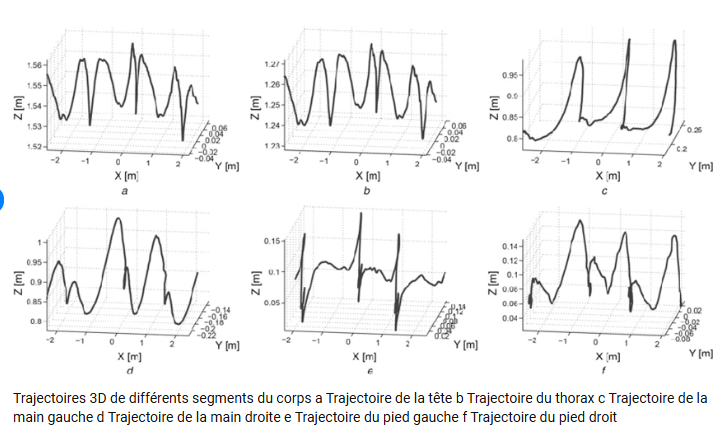
\includegraphics[width=0.5\textwidth]{images/trajectoires_3D.png}
  \end{center}
  \caption{Trajectoires tridimensionnelles de différents segments du corps}\label{fig:trajectoires_tridimensionnelles}
\end{figure}

\subsection{Paramètres spatio-temporels (pistes de marche électronique)}

On cherche à mesurer la \textbf{vitesse moyenne} de la marche ou de la course, ainsi que la \textbf{longueur du pas}, c'est-à-dire la distance parcourue entre deux appuis successifs d'un même pied.
On mesure également la \textbf{cadence} (en unité de temps), et le \textbf{temps de contact au sol}.

Ces données nous permettent d'analyser la marche, ce qui est utilisé pour évaluer la régularité et l'efficacité du mouvement.
Ces données nous assistent aussi dans l'identification des anomalies de la marche liées à des conditions neurologiques, musculo-squelettiques ou orthopédique.o

Ces signaux sont exploités en clinique dans le diagnostic des troubles de la démarche (e.g. après un AVC, ou en cas de maladie de Parkinson).
Elles se révèlent utiles dans le suivi des progrès des patients en rééducation.
Également, l'analyse de la foulée est pratiqué dans le domaine sportif afin d'améliorer les performances des coureurs.

L'analyse de ces signaux est rendue possible par ces machines spécialisées :
\begin{itemize}
  \item \textbf{GAITRite} : fournit des mesures spatio-temporelles précises via des tapis électroniques.
  \item \textbf{Zebris FDM-T} : Intègre la baropodométrie pour une analyse complète de la marche.
  \item \textbf{MotionMetrix}: Capture les paramètres spatio-temporels et les intègre dans une analyse globale du mouvement
\end{itemize}


\begin{figure}[ht]
  \centering
  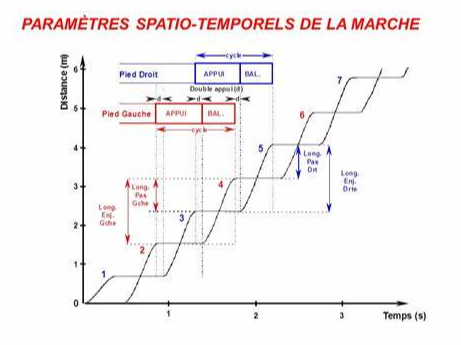
\includegraphics[width=0.5\textwidth]{images/activites_posturo_cinetiques.png}
  \caption{Paramètres spatio-temporels de la marche}\label{fig:parametres_spatio_temporels}
  \label{fig:spatio_temporels_marche}
\end{figure}

\begin{figure}[ht]
  \centering
  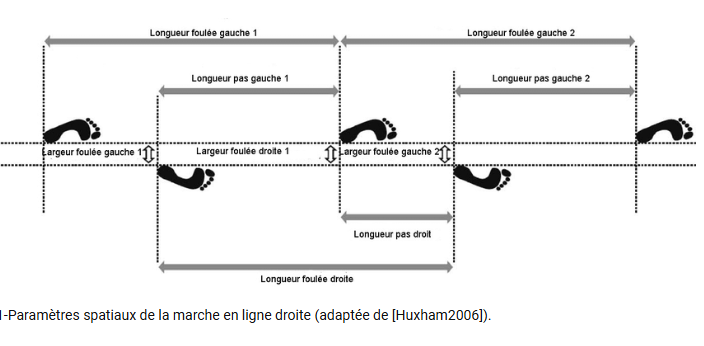
\includegraphics[width=0.5\textwidth]{images/spatio-temporels-ligne-droite.png}
  \caption{Paramètres spatiaux de la marche en ligne droite}
  \label{fig:param_spatiaux_ligne_droite}
\end{figure}
